\documentclass{article}
\usepackage[utf8]{inputenc}
\usepackage{amsmath}
\usepackage{graphicx}
\usepackage{hyperref}
\parindent=0pt
\usepackage[a4paper, total={175mm, 252mm}]{geometry}
\usepackage[section]{placeins}
\usepackage{enumitem}
\usepackage{caption}
\usepackage{parskip}

\title{PySpi for Persistent Sources}
\author{Möller, Julius}
\date{May 2023}

\begin{document}

\maketitle


\tableofcontents

\pagebreak


\section{General Procedure}
In contrast to previous approaches to working with INTEGRAL SPI, this method does not attempt to fit the background via physical models, and instead uses a profile likelihood to eliminate its effect in the source model fit. The underlying assumption that allows this to work is that background count rates in each energy bin remain constant for temporally and spatially near SPI Science Windows (SCWs). Here we distinguish between source counts, which describe all detected events directly originating from astronomical objects considered in our source model and background counts, which describe all other detector events.

This works in the following way: once we have split our set of SCWs into clusters within which we claim the assumption of constant background to be true and have defined a source model, a likelihood value can be calculated for each energy bin of each detector in each cluster. If one energy bin of one detector in one SCW with measuring time $t$ has a source count rate $s$ and a background count rate $b$, the probability $P$ of measuring $C$ counts follows a Poisson distribution:
\begin{equation}
    P(C \vert b, s, t) = \frac{\left( t \left( b + s \right) \right) ^C \text{exp}\left( -t \left( b+s\right)\right)}{C!}
\end{equation}

Equivalent energy bins in the same cluster are assumed to have the same background count rate $b$, so that the probability of measuring $C_1$ counts in one SCW and $C_2$ counts in another SCW is simply:

\begin{equation}
    P(C_1, C_2 \vert b, s_1, t_1, s_2, t_2) = P(C_1 \vert b, s_1, t_1) \cdot P(C_2 \vert b, s_2, t_2)
\end{equation}

The likelihood $\mathcal{L}$ for any energy bin of a detector within a cluster depends on all equivalent energy bins in that cluster, i.e. one term for each SCW in the cluster. If we have cluster of size two, the likelihood is described by:

\begin{equation}\label{log likelihood}
    \text{ln}\mathcal{L}(C_1, C_2, t_1, t_2\vert b, s_1 s_2) = \text{ln}P(C_1 \vert b, s_1, t_1) + \text{ln}P(C_2 \vert b, s_2, t_2)
\end{equation}

This expression allows us to solve for the probability distribution of $b$. A full and mathematically correct treatment of the background parameter $b$ turns out to be very cumbersome with only marginal benefits. Hence, the profile likelihood is used by simply solving for the background count rate value $b_M$ which maximizes the likelihood. This is easily done by setting the derivative of equation \ref{log likelihood} to zero and solving for $b$. For a cluster size of two one finds:
\begin{equation}
    b_M = \frac{1}{2} \left[ \frac{C_t}{t_t} - s_t + \sqrt{\left( \frac{C_t}{t_t} - s_t\right)^2 + 4 \left( \frac{C_1s_2+C_2s_1}{t_t}-s_1s_2\right)}\right]
\end{equation}
where $C_t=C_1+C_2$, $s_t=s_1+s_2$, and $t_t=t_1+t_2$. Using this maximum likelihood background $b_M$ finally allows us to compute a likelihood value that is only dependent on the measured counts and the source model:
\begin{equation}
    \text{ln}\mathcal{L}(C_1, C_2, b_M, t_1, t_2 \vert s_1, s_2) = \text{ln}P(C_1 \vert b_M, s_1, t_1) + \text{ln}P(C_2 \vert b_M, s_2, t_2)
\end{equation}
The process for clusters with sizes larger than two is analogous. One such likelihood value exists for every energy bin of every detector in every cluster, such that the total likelihood value for any given source model is simply the sum of the logarithmic likelihoods over all energy bins, detectors, and clusters. Thus the source model may be fitted to the count data by applying an algorithm to maximize the likelihood.


\section{Spimodfit Procedure}
In order to be able to compare the results obtain using PySpi and the method described above, spimodfit will be used with the same dataset. For the sake of limiting sources of potential errors, the procedure for obtaining results using spimodfit will be described in more detail than might otherwise be deemed necessary. In general, the  \href{https://www-cms.mpe.mpg.de/gamma/instruments/integral/www/}{spimodfit cookbook found here} was followed very closely. In all of the following sections only the SE Data was used by Spimodfit with an energy up to 600keV, compared to a possible 2MeV in the data used by Pyspi. 

\subsection{Fitting the Crab Nebula} \label{Spimodfit crab steps}

\begin{enumerate}
    \item On the ga05us.mpe.mpg.de PC, head into the directory:
    
    \verb|/home/jmoeller/cookbook/SPI_cookbook/examples/Crab|

    \item \label{scw select} In the file \verb|spiselectscw.cookbook_dataset_02_0020-0600keV_SE.par| specify which revolution is to be used via the \verb|fits_revolutions_list| and \verb|revolutions_cond_value| parameters. Run the script:
    
    \verb|./submit-spiselectscw_ga05us.sh cookbook_dataset_02_0020-0600keV_SE &|

    \item \label{step background} In the file \verb|background_model_SE_02.pro| change the parameters \verb|spidir|, \verb|scw_file|, and \verb|bgdir| to point towards the correct directories in the newly created directory \verb|cookbook_dataset_02_0020-0600keV_SE|. Run this script: 
    
    \verb|idl idl-startup.pro background_model_SE_02.pro|

    \item \label{Source directory} In the file \verb|spimodfit.fit_Crab_SE_02.par| change the parameters \verb|counts_input_file|, \verb|pointing_input_file|, \verb|ebounds_input_file|, \verb|deadtime-dol|, \verb|gti-dol|, and \verb|background_input_file| to point to the correct directories. Furthermore, specify the source catalogue directory:
    
    \verb|source-cat-dol,s,h,"/home/jmoeller/cookbook/SPI_cookbook/cats/cat_crab.fits.gz"|

    Leave everything else untouched and run the script:

    \verb|./submit-spimodfit_v3.2_ga05us.sh fit_Crab_SE_02 clobber &|

    \item \label{Spectrum file} Inside the directory \verb|fit_Crab_SE_02| run the script \verb|./spimodfit_rmfgen.csh|. Back in the previous directory, edit the parameters \verb|response_file| and \verb|spectrum_file_01| in the file \verb|adjust4threeML_SE_02.pro| to point at the correct directories, and run the script:
    
    \verb|idl idl-startup.pro adjust4threeML_SE_02.pro|

    \item For convenience, transfer the files \verb|specra_Crab.fits| and \verb|spectral_response.rmf.fits| onto local machine. Here the script found in
    
    \verb|/home/jmoeller/cookbook/SPI_cookbook/spectral_analysis/3ml_fit_Crab_SE.py|
    
    is used extract the fit parameters, where the source model can be changed and active measurements (i.e. energy range) can be changed as pleased.
\end{enumerate}


\subsection{Fitting other Sources}
If we want to fit another source instead of the Crab, the following changes are made to the previously described steps:

\begin{enumerate}
    \item Access the SPI source catalogue: \verb|/home/jmoeller/cookbook/SPI_cookbook/cats/spi_cat.fits.gz|
    \item Create a new file with only one (or more, depending on how many sources we want to fit) row from the source catalogue, representing one source. Edit the entries \verb|RA_OBJ|, \verb|DEC_OBJ|, and \verb|NAME| to the coordinates and name of the new source. Other entries in the row are not used and irrelevant for the fit.
    \item Place the new file in the same directory as the original catalogue.
    
    Now repeat steps from section \ref{Spimodfit crab steps} with the following differences:
    \item In step \ref{scw select} from section \ref{Spimodfit crab steps} also change the parameters 
    
    \verb|select_PtgX_masks_chi_list_1| and \verb|select_PtgX_masks_psi_list_1| 
    
    to the coordinates of the new source. Note that these are galactic coordinates.
    \item In step \ref{Source directory} from section \ref{Spimodfit crab steps} change \verb|source-cat-dol| to instead point to the new source file.
    \item The new spectrum output file will be names according to the new source name, which has to be reflected in the parameter \verb|spectrum_file_01| from step \ref{Spectrum file} in section \ref{Spimodfit crab steps}.
\end{enumerate}


\subsection{Fitting Custom Data}
If we want to use Spimodfit to fit our own custom data, for example for simulated sources, we can once again repeat the steps from section \ref{Spimodfit crab steps} with one difference. After step \ref{scw select} is completed the directory

\verb|/home/jmoeller/cookbook/SPI_cookbook/examples/Crab/cookbook_dataset_02_0020-0600keV_SE/spi|

is created, which includes the relevant data files to be used in the fit. Here we can edit \verb|evts_det_spec.fits.gz| to our custom data, which obviously has to take into consideration which SCW, detector, and energy bin each table entry corresponds to. 


\subsection{Spimodfit Background} \label{spimodfit bkg}
For every fit, Spimodfit creates a background model. After step \ref{step background} in section \ref{Spimodfit crab steps} is completed the directory

\verb|/home/jmoeller/cookbook/SPI_cookbook/examples/Crab/cookbook_dataset_02_0020-0600keV_SE/|\newline
\verb|spi/bg-e0020-0600|

is created, containing the files \verb|output_bgmodel-conti.fits.gz| and \verb|output_bgmodel-lines.fits.gz|. These contain the expected number of counts for each energy bin from each detector in each SCW. In order to obtain a usable background model one can Poisson distribute the files and then add them together. Since some elements are negative, one can take the Poisson distribute the absolute values and multiply the result with the sign of the original number. 



\section{Results: Crab Nebula}

\begin{figure}[h]
    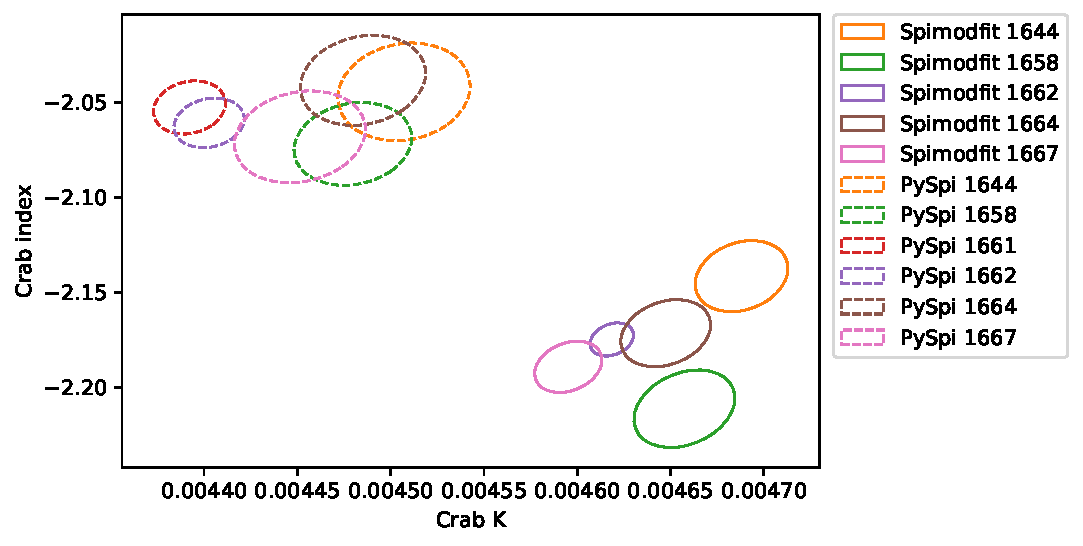
\includegraphics[width=\textwidth]{Images/crab_ps_smf_wo_out.pdf}
    \caption{}
    \label{Crab}
\end{figure}

Figure \ref{Crab} shows one standard deviation confidence intervals of several near SPI Revolutions, as fitted using PySpi and Spimodfit. Revolution 1661 was only fitted using PySpi since spimodfit rejected all SCWs due to "General Expression". The source model is a simple powerlaw 
\begin{equation} \label{powerlaw}
    f(x) = K \frac{x}{piv}^{index}
\end{equation}
where $K$, measured in $\text{keV}^{-1}\text{s}^{-1}\text{cm}^{-2}$ is the differential flux at the pivot value $piv=40$keV, $x$ is the photon energy in keV, and $index$ is the index of the powerlaw.

Both methods used the same energy range of 20-81.5keV, although it is worth pointing out that they use independent algorithms to select which SCWs are used in the fit. PySpi used a cluster size of two. 

Although the two methods obtain different values for the index and normalization, we see comparable sizes of uncertainties as well as similar levels of compactness within the values from different revolutions. 

The data used by PySpi was also subjected to a Posterior Predictive Check (PPC) analysis, allowing for revolution pairs that did not match the source model to be manually removed. This substantially improved the consistency of the fits.

\section{Results: Simulated Source}
The downside to fitting a real astronomical object such as the Crab nebula is that one can never be exactly sure what the true source parameter values should be. This is why it can be advantageous to simulate a source, feed the simulated data back into the fit, and compare the produced source parameters to the now known true values.

However, not only a simulated source is required, but a background as well. There are different approaches one may take to realize this. The first approach is to use an entirely real dataset from a SPI revolution as background, and add a simulated source on top:

\begin{enumerate}
    \item \label{step bkg}Choose a data set to use as background. This was done once with real data, in this case a single SPI revolutionFor this to work well, there should be as few bright sources within the field of view as possible, since these will interfere with the fit if not included in the source model. This step was also performed using the Spimodfit background spectrum, as described in section \ref{spimodfit bkg}. Alternatively, one can also use a constant background spectrum for all SCWs. This may be realized by choosing one SCW and duplicating its counts to all other SCWs. The counts have to be  redistributed according to a Poisson distribution and the lifetimes of the other SCWs has to be adjusted as well. 
    
    \item Define spectrum of the source to be simulated, as well as position. In this case powerlaws as shown in equation \ref{powerlaw} are used, and the position of the sources is chosen to be central to as many SCWs in the revolution as possible.
    
    \item Use the SPI Instrument Response Function (IRF) to calculate the expected source count rates in each energy bin in each detector for each SCW. Multiply by these be the respective lifetime (effectively the active measuring time) of the detector in the SCW, and finally draw a sample of a Poisson distribution with the respective means to attain the measured counts of the simulated source for each energy bin in each detector in each SCW.
    
    \item These source count rates are then added to the background spectrum to acquire the total counts.
\end{enumerate}

This dataset can then be used to fit the simulated source with both PySpi and Spimodfit. When using real data in step \ref{step bkg} this method produces a very realistic background, which in some cases it may be too realistic by including unwanted sources in the field of view that interfere with the fit. This is why it can be beneficial to use the Spimodfit background spectrum or a constant background spectrum instead. The results of this for revolutions 0374 and 1380 are shown in figures \ref{0374 sim source} and \ref{1380 sim source}. Spimodfit was not given the data with a constant background spectrum, since its approach to modelling the background does not allow it to deal with arbitrary spectra. 

\begin{figure}[h]
    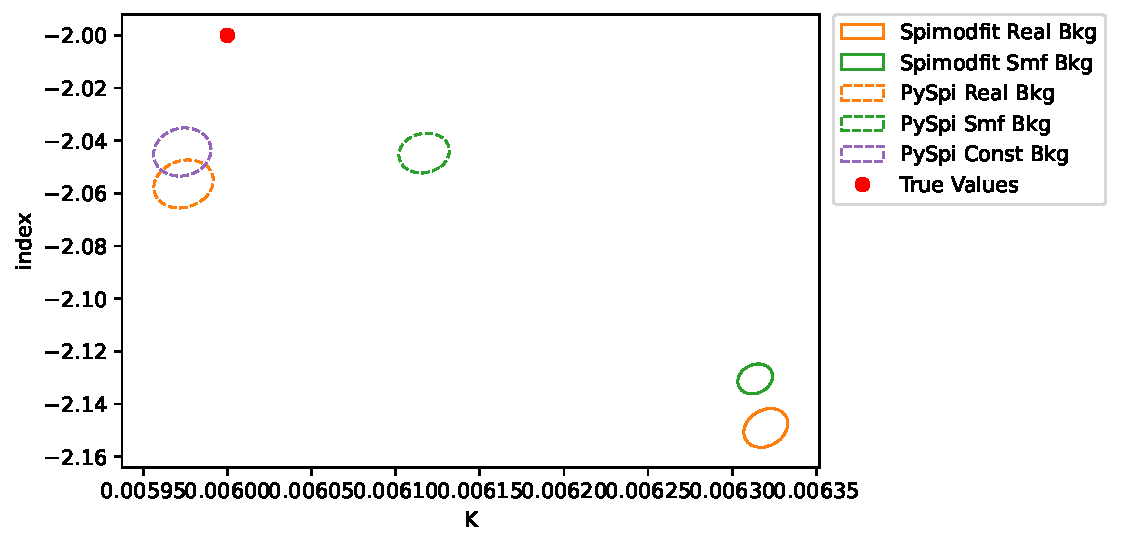
\includegraphics[width=\textwidth]{Images/0374_sim_source.pdf}
    \caption{Simulated Powerlaw source with $K=0.006\text{keV}^{-1}\text{s}^{-1}\text{cm}^{-2}$, $piv=40\text{keV}$, and $index=-2$ for the different methods of generating a background spectrum fitted using PySpi and Spimodfit. This is based on revolution 0374 with the equatorial coordinates of the source at $RA=10, DEC=-40$. As always, the ellipses show the confidence intervals of one standard deviation.}
    \label{0374 sim source}
\end{figure}

\begin{figure}[h]
    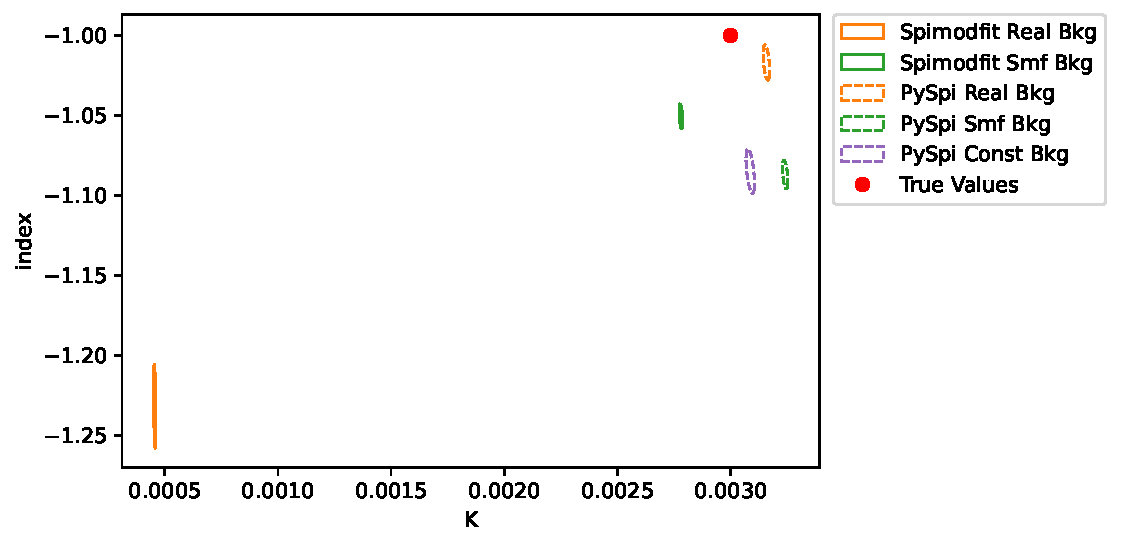
\includegraphics[width=\textwidth]{Images/1380_sim_source.pdf}
    \caption{Simulated Powerlaw source with $K=0.003\text{keV}^{-1}\text{s}^{-1}\text{cm}^{-2}$, $piv=40\text{keV}$, and $index=-1$ for the different methods of generating a background spectrum fitted using PySpi and Spimodfit. This is based on revolution 1380 with the equatorial coordinates of the source at $RA=155, DEC=75$.}
    \label{1380 sim source}
\end{figure}

In general we see PySpi consistently perform better than Spimodfit. A couple of curious results stand out. One is that PySpi performs consistently worse with the Spimodfit background spectrum. In theory, one might not expect this since the Spimodfit background spectrum should not include any point sources in SPIs field of view, so that the fundamental assumption of constant background in SCW clusters should be well met. Another curiosity is that the effect of using Spimodfit with the data produced using the Spimodfit background spectrum has inconsistent results. For revolution 0374 this makes almost no difference to using the real data as background, where as in revolution 1380 the results improve dramatically. Finally, it is very curious how PySpi with a constant background spectrum does not perform as well as one might expect, since the fundamental assumption of constant background is perfectly met. This demonstrates systematic inaccuracies with the PySpi approach to fitting, which are further explored in section \ref{sec: pure sim}.

\begin{figure}[h]
    \centering
    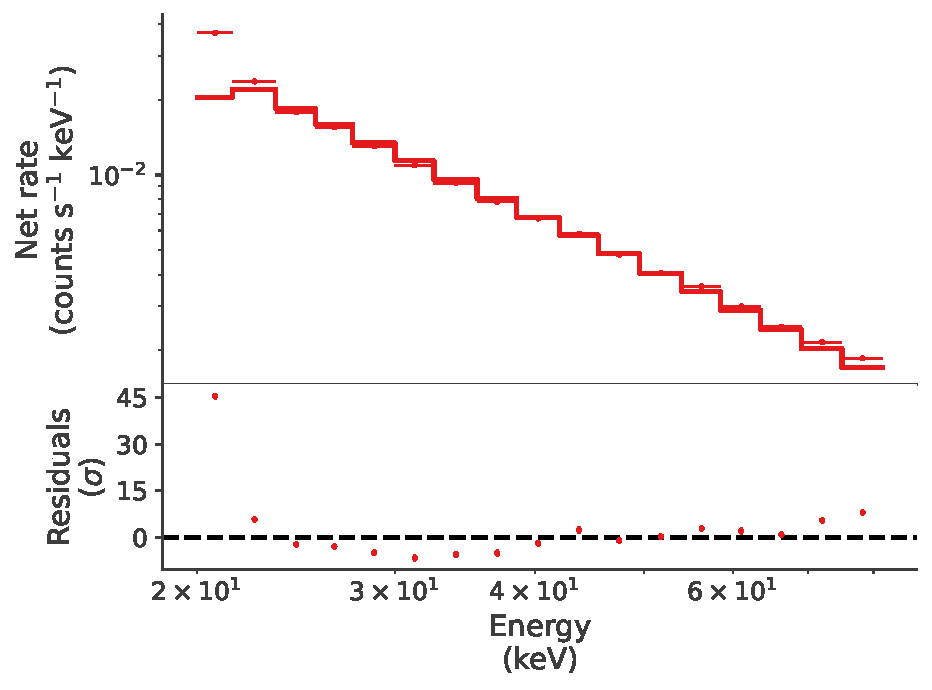
\includegraphics[width=0.7\textwidth]{Images/smf_spec_0374_sim_source.pdf}
    \caption{Spimodfit spectrum and source model for revolution 0374 using the simulated source and the real background spectrum.}
    \label{smf_spec_0374}
\end{figure}

\begin{figure}[h]
    \centering
    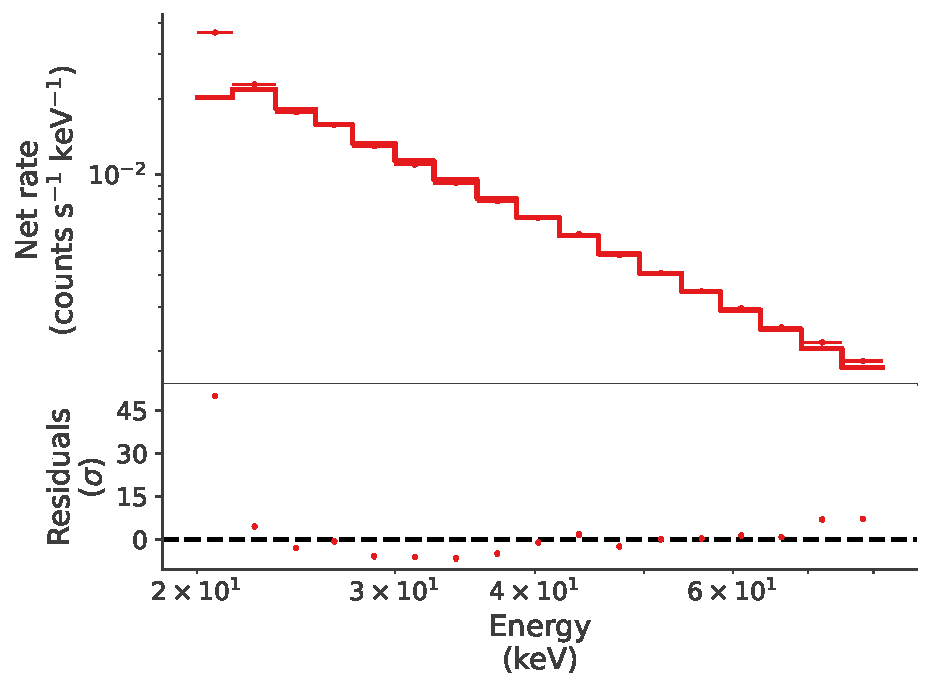
\includegraphics[width=0.7\textwidth]{Images/smf_spec_0374_sim_source_smf_bkg.pdf}
    \caption{Spimodfit spectrum and source model for revolution 0374 using the simulated source and the spimodfit generated background spectrum.}
    \label{smf_spec_0374_smf_bkg}
\end{figure}

\begin{figure}[h]
    \centering
    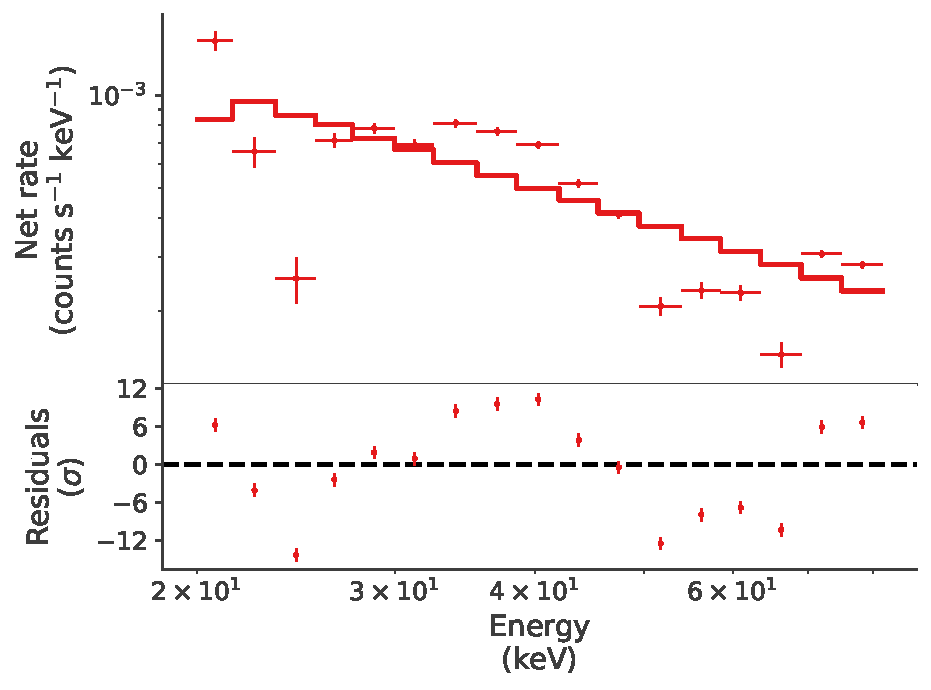
\includegraphics[width=0.7\textwidth]{Images/smf_spec_1380_sim_source.pdf}
    \caption{Spimodfit spectrum and source model for revolution 1380 using the simulated source and the real background spectrum.}
    \label{smf_spec_1380}
\end{figure}

\begin{figure}[h]
    \centering
    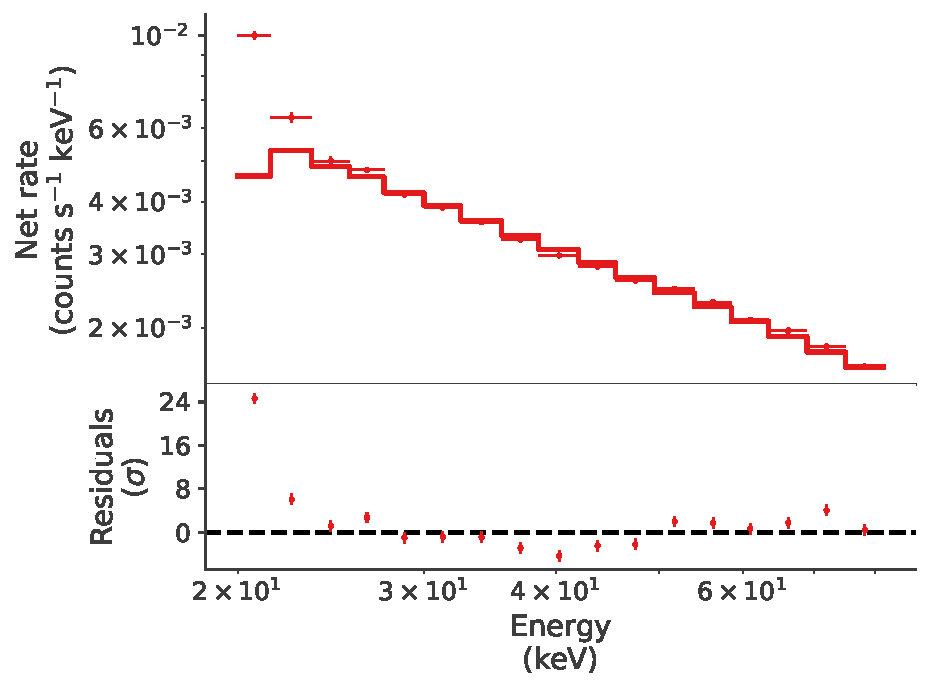
\includegraphics[width=0.7\textwidth]{Images/smf_spec_1380_sim_source_smf_bkg.pdf}
    \caption{Spimodfit spectrum and source model for revolution 1380 using the simulated source and the spimodfit generated background spectrum.}
    \label{smf_spec_1380_smf_bkg}
\end{figure}


Finally, the count and source model spectra produced by the Spimodfit fits are shown in figures \ref{smf_spec_0374} to \ref{smf_spec_1380_smf_bkg}. Two possible signs of errors are the first energy bin is always significantly higher than predicted by the source model, and that the uncertainties for revolution 1380 with real background data are very high.

\section{Background Analysis}



\begin{figure}[h]
    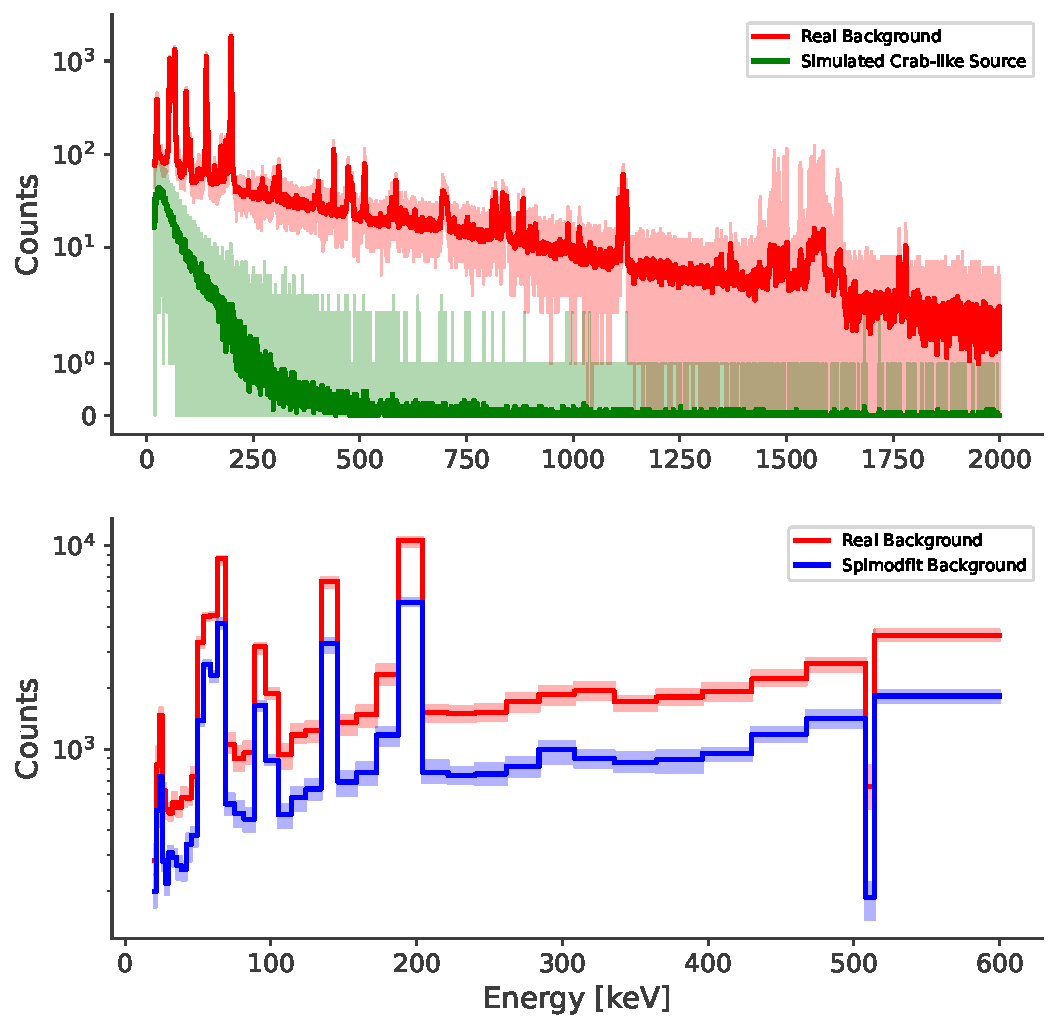
\includegraphics[width=\textwidth]{Images/background.pdf}
    \caption{Background spectrum of SCW 03740002 in comparison to count rates from a simulated source with a powerlaw spectrum similar to that of the Crab nebula. In the bottom plot, the spectrum is rebinned so that it may be compared to the spimodfit background spectrum of the same SCW. The shaded areas show the range over all detectors, whereas the solid line shows the mean over all detectors.}
    \label{plt bkg spec}
\end{figure}

The counts from SCW 03740002 are used very often as an example background spectrum, and duplicated to other SCWs in the revolution for a constant background. Hence, it can be beneficial to visualize this spectrum, as was done in figure \ref{plt bkg spec}. Two things worth noting are that the counts from the simulated Crab-like source are significantly lower than those from the background, especially at higher energies, and that the Spimodfit background spectrum, although very similar in shape, is consistently lower than the real background by a roughly constant factor.

\begin{figure}[h]
    \centering
    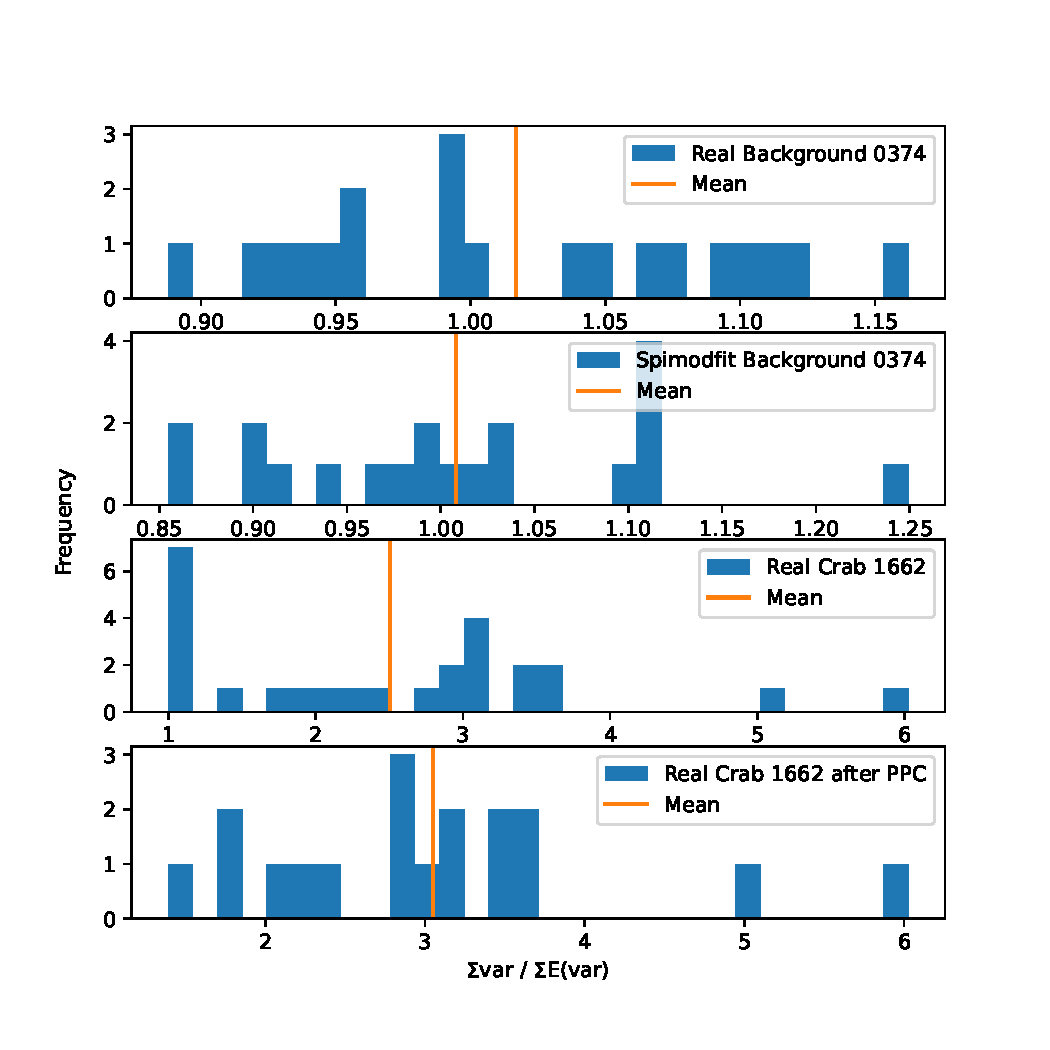
\includegraphics[width=0.9\textwidth]{Images/background_variance.pdf}
    \caption{A histogram of the ratio of the variances to the expected variances based of the SCW clusters for different data sets. (see text)}
    \label{plt bkg var}
\end{figure}

While we are analyzing data spectra that we consider to be background-like (i.e. no point-like source in SPIs field of view), there is a very insightful statistical test we can do. After pairing up SCWs into clusters within a SPI revolution, we can calculate the variance of the counts in each energy bin of each detector of each SCW cluster, and then compare this to the variance we would expect if the two counts were Poisson sampled based on a common underlying background count-rate. The definition of the Bessel corrected variance of the two counts is standard, and the expected variance is also relatively straightforward to compute given the fact that variances of independent distributions add together:

\begin{equation}
    E(var) = (rt_1 - m)^2 + (rt_2 - m)^2 + \frac{r(t_1+t_2)}{2}
\end{equation}

where $r=\frac{C_1+C_2}{t_1+t_2}$ is the average count-rate in both energy bins, $m=\frac{C_1+C_2}{2}$ is the average number of counts, and $t_1$ and $t_2$ are the lifetimes of the respective SCWs. We may then sum the variance and expected variance over all energy bins and all detectors for each cluster of SCWs and take their ratio to get an estimate of how well the fundamental assumption of a constant background count-rate within SCW clusters is met. A ratio $var / E(var)$ around 1 means that the variances between the two SCWs are entirely explained by Poisson sampling with a common count-rate, in comparison to a ratio larger than 1 indicating a source in SPIs field of view, hence non-common count-rates for identical energy bins in the clustered SCWs.

This was plotted in figure \ref{plt bkg var} for the real data from revolution 0374 and the Spimodfit generated background spectrum for revolution 0374. We see that both are closely distributed around 1, meaning that the fundamental assumption of constant background rates within SCW clusters is well met, both within the real data and the spimodfit generated background. 

Additionally, the same analysis was performed on revolution 1662, featuring many SCWs with the Crab Nebula within 10 degrees of the center of SPIs field of view. As expected, we see that the ratio of the variances is now considerably higher. Curiously, there are still several clusters with a ratio close to 1, implying that there are no visible sources in SPIs field of view. Since the Crab nebula is always within 10 degrees of the field of view, this is impossible. It is unclear what happened in these SCW clusters, but whatever the cause, any sources are completely drowned out. A PPC analysis was conducted on this revolution, with notable outlier SCW clusters being removed from the fit. As expected, this removes exactly those SCW clusters with a variance ratio close to 1. This highlights the importance of performing a PPC analysis when using PySpi.

\section{Results: Pure Simulation} \label{sec: pure sim}

\subsection{Consistency}

\subsubsection{Dynamic Binning}

\subsection{Different Powerlaws}

\subsection{A Second Source}

\subsection{Energy Range}

\subsection{Number of Energy Bins}

\subsection{Cluster Size}

\end{document}